\chapter{Mars Express, MARSIS and ionograms}

\section{Mars Express}
First of all, let us briefly introduce the spacecraft carrying all the equipment needed to acquire ionograms. Its name is \textit{Mars~Express} (MEX) and it was launched by the \textit{European Space Agency} (ESA) on 2~June~2003.

MEX arrived to Mars at its orbit with periapsis 250~km and apoapsis over 11000~km on~25~December~2003~\citep{Chicarro2004} with seven~onboard scientific instruments and a~landing module called Beagle~2. We're going to take a look at all of them in the following subsections; just Beagle~2 description is going to be rather short, because the landing sequence failed (for an unknown reason) and the lander didn't establish connection after it landed (if it landed at all)\citep[p.~4]{Chicarro2004}. 

The mission of MEX has several goals like ``global studies of the surface, subsurface and atmosphere at unprecedented spatial and spectral resolutions'' \citep[p.~viii]{Chicarro2004}. One of the goals, however, stands out among all the others. It is the search for water (or its traces) on Mars' surface or subsurface.

\begin{figure}
	\centering
	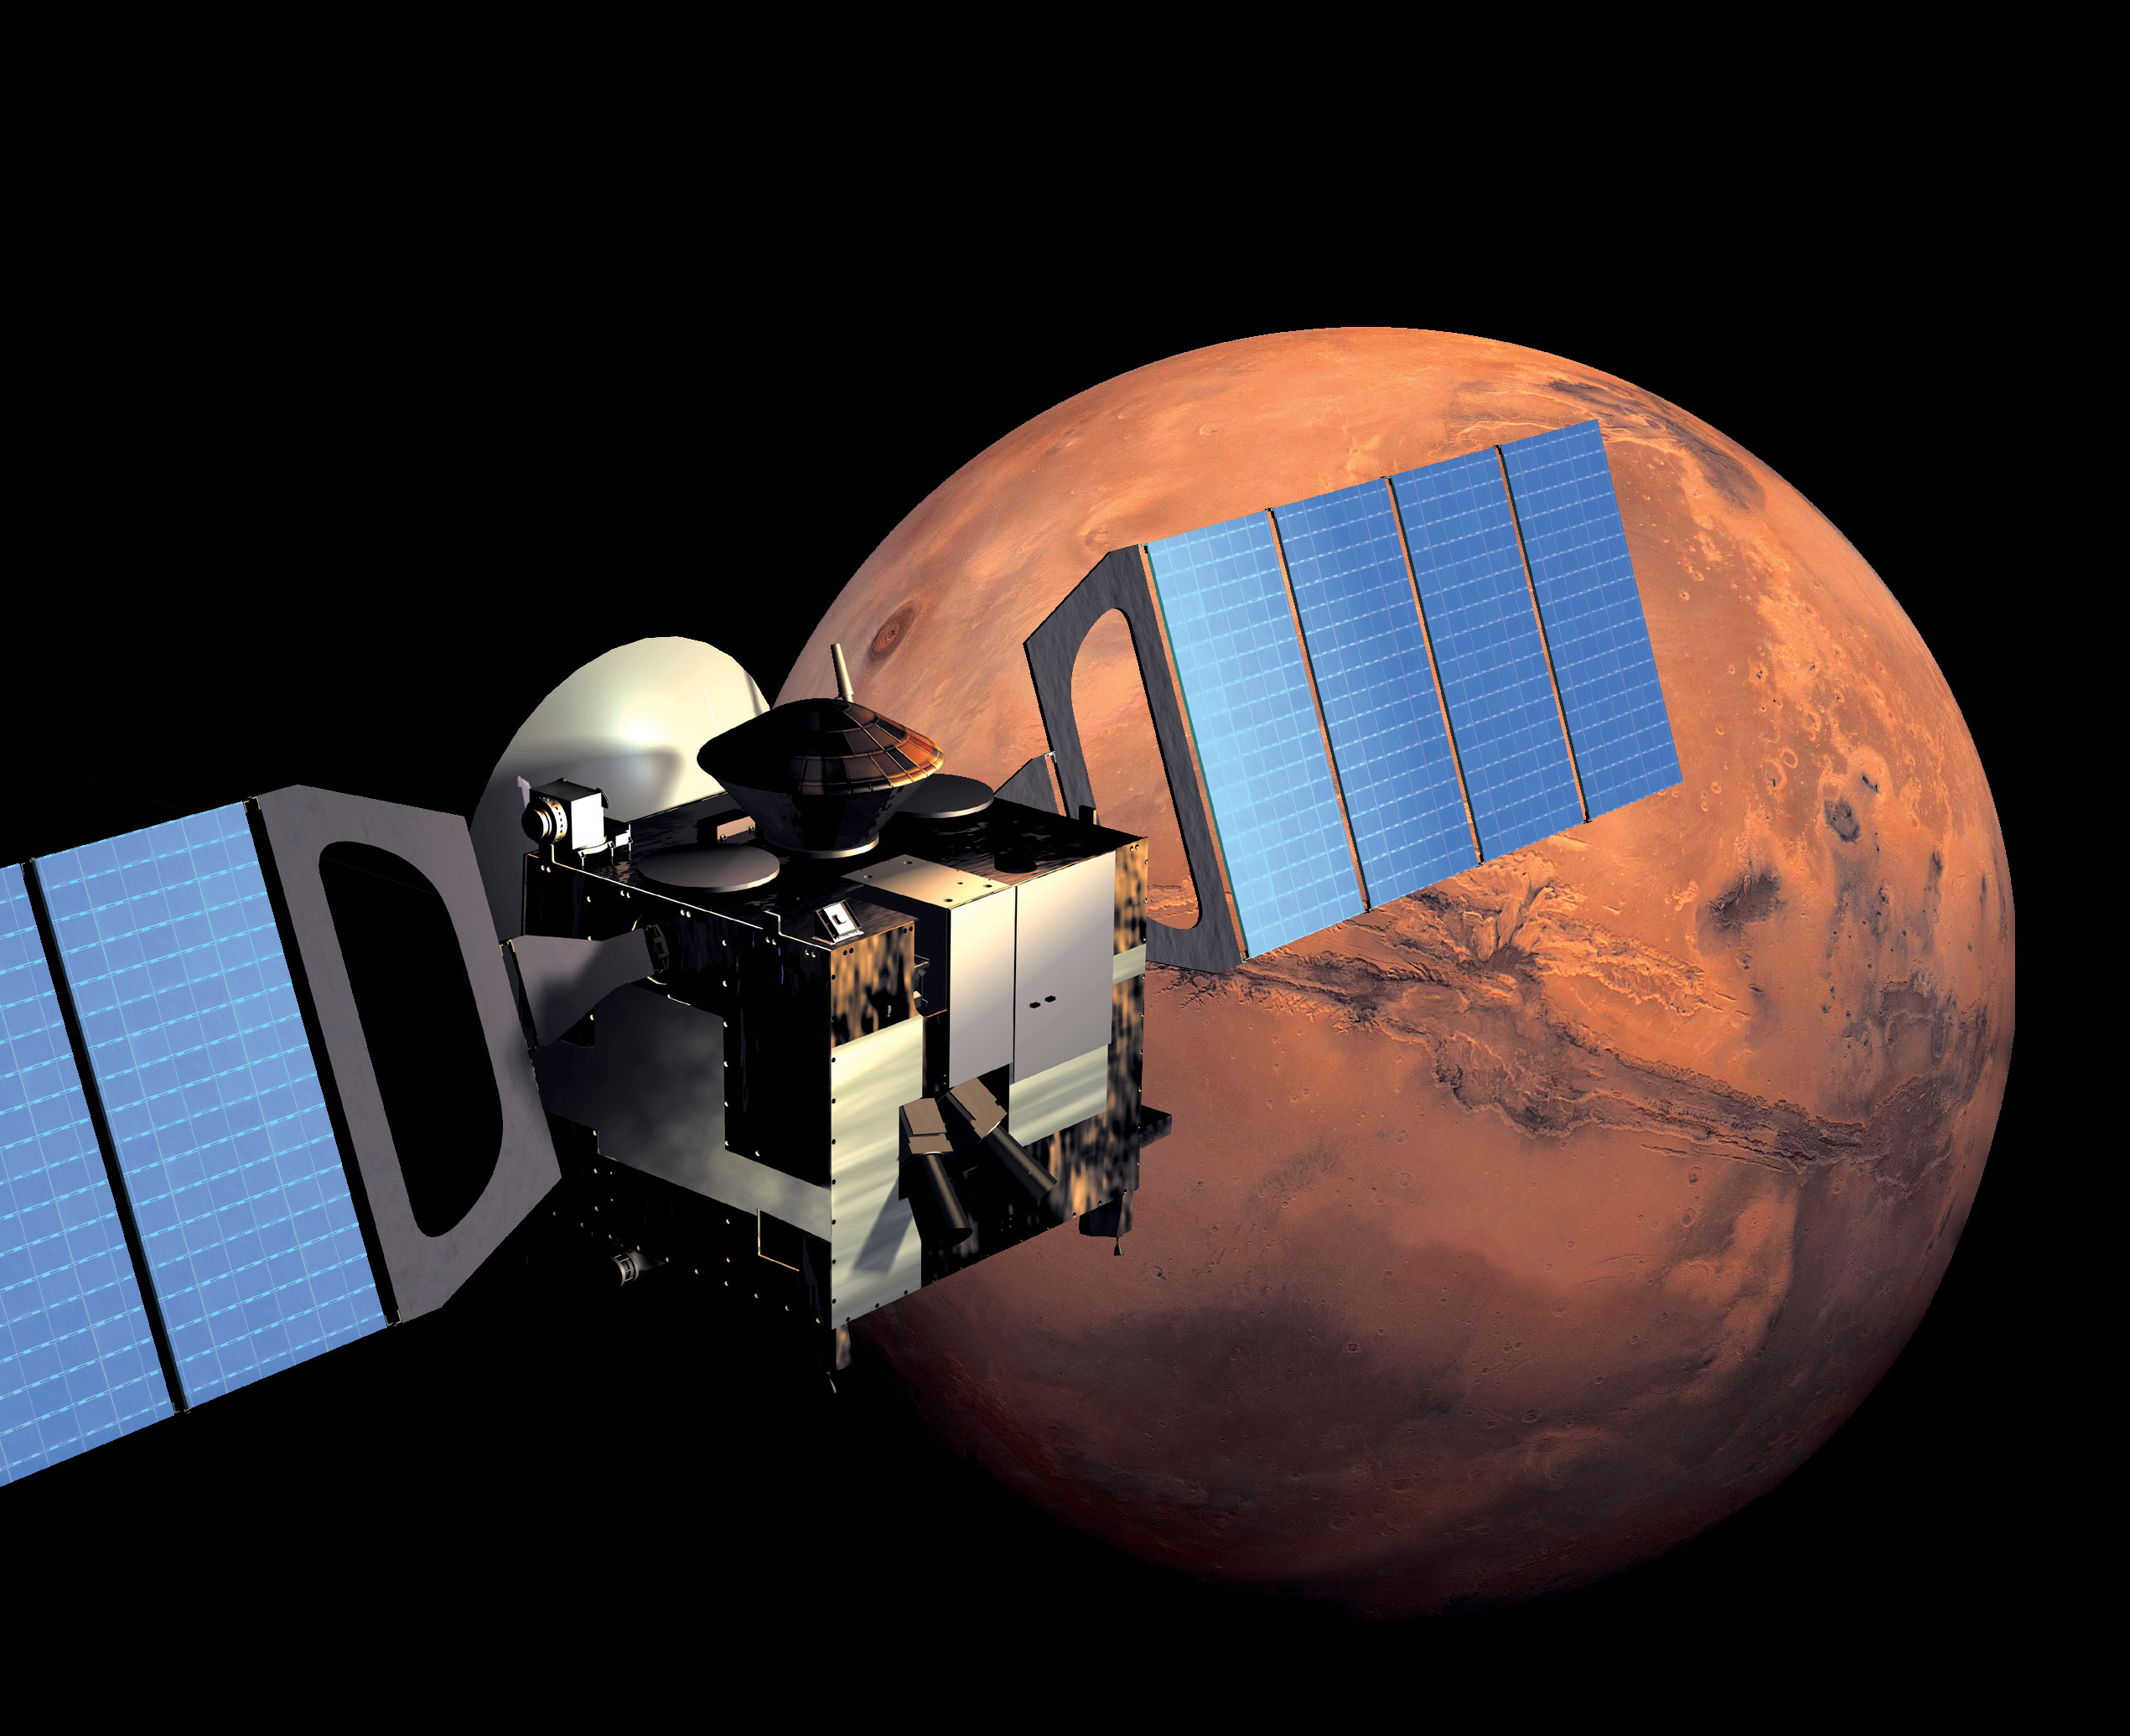
\includegraphics[width=140mm]{images/Mars.jpg}
	\caption{Mars Express spacecraft. Credit: ESA \citep{ESA2010}}
	\label{fig:mex}
\end{figure}

Why water? There is lots of geological evidence of former water occurrence. But before the~MEX~mission nobody had proved or refuted presence of water on~Mars in the present. Knowing more about water on Mars and its history, the scientists could postulate better hypotheses about the possibility of (former) life on the~planet \citep[p.~ix]{Chicarro2004}. \pdfcomment{Tady si nejsem uplne jisty tim, jak uvadet citace, protoze prakticky cela podkapitola cerpa z jedine knizky}

The original mission lifetime of MEX was projected up~to the~end of~2005 (which would be 1~Martian~year = 687~Earth~days) \citep{ESA2004}. However, overcoming some small problems (as the Solid State Mass Memory anomalies described in~\citep{ESA2011} or the~MARSIS~antennas deployment problems in~2004~\citep{ESA2004a,ESA2005}), MEX has worked on its science goals up to this day and its science mission was extended until~2014~\citep{ESA2013} (after 3~preceding similar extensions). Fred Jansen, MEX mission manager, said MEX had enough fuel for another 14~years of~operation (at the~beginning of~2012)~\citep{Clark2012}. So there is a hopeful prospect of further and even deeper Mars exploration (eg. \citep{Gurnett2005}~discovered an~unexpected way of~using the MARSIS~instrument so that they ``added magnetometer functionality'' to~MARSIS).

In the~next subsections you can find~out more about particular MEX instruments. The descriptions are based on~\citep{Chicarro2004} which you can see for~more detailed information.

\subsection{HRSC (\textit{High--Resolution Stereo Camera})}

\begin{figure}
	\centering
	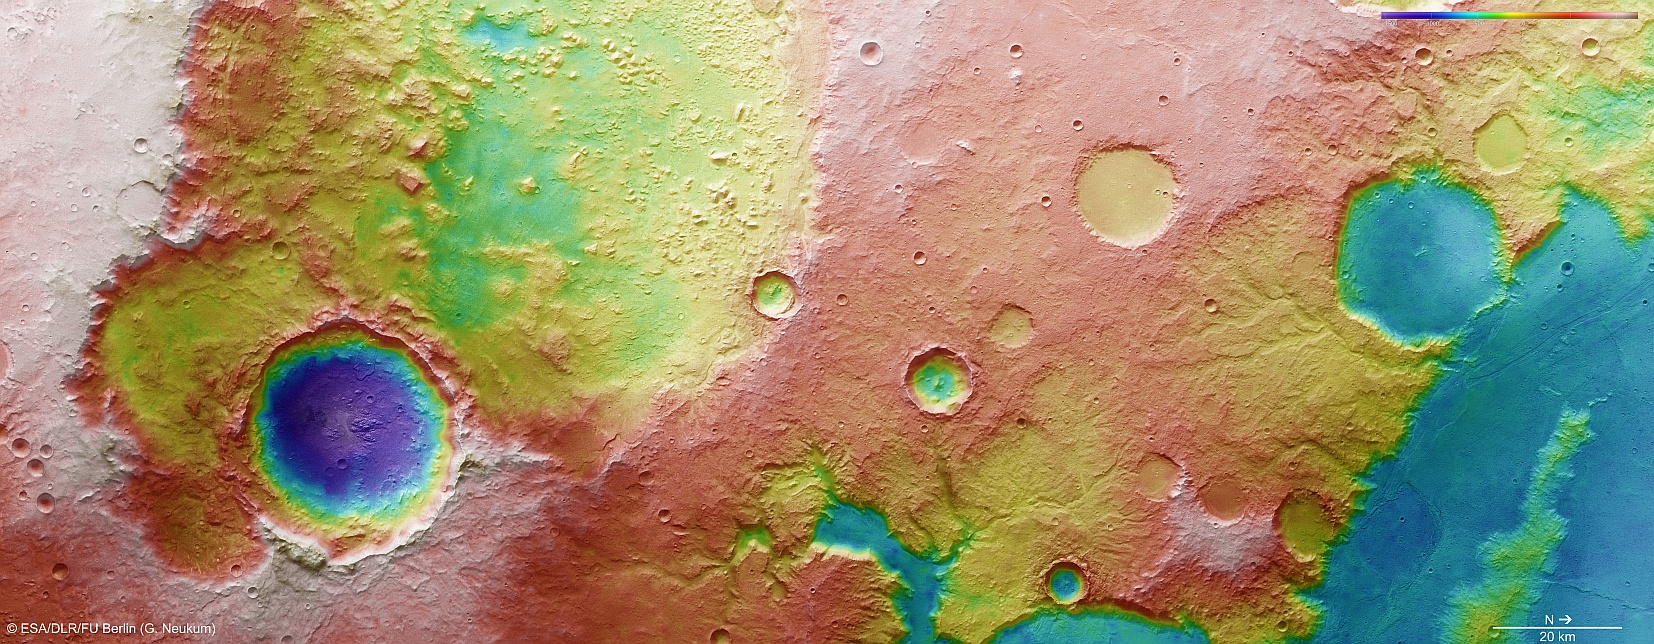
\includegraphics[width=140mm]{images/Topographical_view_of_Amenthes_Planum.jpg}
	\caption{Example image taken by HRSC. Credit: ESA/DLR/FU Berlin (G. Neukum) \citep{Neukum2013}}
	\label{fig:hrsc_example}
\end{figure}

HRSC is a~high--resolution pushbroom\footnote{A camera that scans the image by rows perpendicular to the flight direction. See \url{http://earthobservatory.nasa.gov/Features/EO1/eo1\_2.php} for more details.} camera for~surface imaging. Its goals are to~characterize surface structure and morphology at~resolution 10~m~px$^{-1}$ (regions of interest at 2~m~px$^{-1}$), surface topology at high vertical resolution, atmospheric phenomena, physical properties of the~surface and to~classify terrain and to~refine the~martian cartographic base. It is also intended to observe Mars' moons Phobos and Deimos during their approaches.

HRSC is~able to capture the surface at~resolution up~to~10~m~px$^{-1}$ with field of~view~11.9�, covering a 52.2~km wide strip of surface at~height 250~km (which is the~periapsis of~MEX). The camera consists~of 9~CCD~sensors allowing it to acquire triple stereo images in 4~colors and 5~phase angles. What is a very useful property of these images, is that they are taken nearly simultaneously and thus having the same illumination and other observational conditions (which further helps in photogrammetric processing of the images).  

HRSC also contains a~super--high--resolution camera called~SRC (\textit{Super--Resolution Channel}) aimed at~targeted observations of~particular surface details. With image resolution 2.3~m~px$^{-1}$ and field of view 0.54� it provides a detailed view of a 2.3x2.35~km large surface. Its main purpose is to~take details of~places of~interest, eg. future landing sites for other landing modules.

% achievements
Up to November~2011 HRSC had covered about~88\% of the martian surface \citep[pp.~72--73]{ESA2011a} and still continues to gather new data. The scientific results of HRSC are for example better exploration of fluviatile valleys \citep{Mangold2008}, dicovery of numerous glacial landforms, investigating lava flows, dicovery of ``dust devils'' (fast moving dust storms) or providing data to derive a detailed topographic model of more than 20\% of Phobos \citep[pp.~945--949]{Jaumann2007}.

\subsection{OMEGA (\textit{Observatoire pour la Min�ralogie, l'Eau, les Glaces et l'Activit�})}
OMEGA is a medium-- and high--resolution spectrometer operating in~visible and near--IR spectra (0.38--5.1 $\upmu$m wavelength). Its medium--resolution operating mode (from heights of~1500 to~4000~km) can measure with the resolution~2--5~km targeting at global surface coverage, while the high--resolution~mode (from the~close vicinity of~periapsis) brings resolution 350~m or~better, but will cover only a small fraction of the surface. 

As stated in~\citep[pp.~38--39]{Chicarro2004}, the main goals are to~study the~evolution of~Mars, to~detect minerals hidden to~lower resolutions, to~map mineralogical boundaries between geological units, to~reveal gradients in hydration minerals related to~fossil water flows and to~monitor features associated with~wind transportation. In~particular, it is intended to find carbonates (not found on martian surface until the launch of MEX) and water ice. It is also able to measure atmospheric pressure, CO and H$_2$O column densities and surface temperature.

Recent contributions of the OMEGA payload are e.g. confirmation of liquid water on the surface when the planet was young \citep{Loizeau2012}, discovery of infrared and ultraviolet glows in the atmosphere \citep{Bertaux2012}, proving that Mars had a hot and wet period \citep{Chevrier2007} (implying there were lots of greenhouse gases and a strong magnetic field, too \citep[p.~90]{Fletcher2009}), analyzing the south polar cap and finding out it is formed mainly of water ice \citep{Doute2007}, observation of CO$_2$ ice clouds \citep{Montmessin2007} or finding ferric oxides near the equator \citep{Masse2008}.

\subsection{MARSIS (\textit{Mars Advanced Radar for Subsurface and Ionosphere Sounding})}
MARSIS is a long--wavelength radar using coherent wide-band pulses for sounding of the surface, subsurface and ionospehere of Mars. For these purposes it~uses a 40~m dipole antenna (for both transmitting and receiving) and a~shorter 7~m monopole antenna (only for~receiving). Due to the used sounding frequencies ranging from 100~kHz to 5.5~MHz it is able to reach the depth about 5--8~km under the~surface.

The primary goal of MARSIS is to detect liquid and solid water in the upper crust of Mars. There are also other objectives: subsurface geologic probing (to make a~3D characterization of the subsurface structures), surface characterization (to measure surface roughness, reflectance to radar signals and to estimate topography) and ionosphere sounding (to measure interaction between solar wind and the ionospehere).

To name some results of the MARSIS instrument, we can mention revealing the layered subsurface structure of both polar caps (strongly suggesting there were oceans in distant history at these places) \citep[pp.~98--102]{Fletcher2009} along with estimating the volume of subsurface water ice in the~polar cap \citep{Phillips2008}, discovery of Medusae Fossae Formations (the youngest surface deposits) \citep[pp.~102--105]{Fletcher2009} or mapping the ionosphere and verifying the ionospheric density models \citep[pp.~105-110]{Fletcher2009}.

One surprising and unexpected utilization of the MARSIS instrument is given by the electron cyclotron echoes found in ionograms (see section \ref{ssec:cyclotronEchoes}). It was found that often they correspond to the strength of the magnetic field, effectively allowing to measure that field and compare it to its model. Another type of echoes, the oblique ionospheric echoes (see section \ref{ssec:oblique}) were identified to correspond to the crustal magnetic field. Both these contributions were made by \citep{Gurnett2005}. 

\subsection{PFS (\textit{Planetary Fourier Spectrometer})}

\subsection{SPICAM (\textit{SPectroscopy for the Investigation of the Characteristics of the Atmosphere of Mars})}

\subsection{ASPERA (\textit{Analyser of Space Plasmas and EneRgetic Atoms})}

\subsection{MaRS (\textit{Mars Express Orbiter Radio Science})}

\subsection{Beagle 2}

\section{MARSIS}

\section{Ionograms}

\subsection{Electron cyclotron echoes}
\label{ssec:cyclotronEchoes}

\subsection{Oblique ionospheric echoes}
\label{ssec:oblique}